\PassOptionsToPackage{dvipsnames}{xcolor}
\documentclass[14pt]{beamer}

\usepackage{amsmath}
\usepackage{mathtools}
\usepackage{emoji}
\usepackage{xfrac}
\usepackage{cancel}
\usepackage{csquotes}
\usepackage{array} % need to be explicitly loaded to do advanced column layout
\usepackage{mathrsfs}
\usepackage{listings}
\lstdefinestyle{Matlab}{%
  language=matlab,
  basicstyle=\scriptsize\ttfamily,
  breaklines=true,
  commentstyle=\color{gray},
  showstringspaces=false,
  tabsize=4
}

\usepackage{algpseudocode}

\usepackage[]{xcolor}
\def\MyGreen{ForestGreen}
\def\MyRed{Red}
\def\MyOrange{BurntOrange}
\def\MyBlue{NavyBlue}
\definecolor{SuperLightGray}{rgb}{0.9,0.9,0.9}

\usepackage{calc}

% This lets us \includestandalone tikz pictures in standalone documents.
\usepackage{tikz}
\usetikzlibrary{tikzmark}
\usepackage[mode=buildnew]{standalone}
\usepackage{xifthen}

\makeatother
\renewcommand{\thefootnote}{
    \ifcase\value{footnote}
        \or*
        \or**
        \or***
        \or****
    \fi}
\makeatletter

\usefonttheme{serif}
\setbeamertemplate{navigation symbols}{}%remove navigation symbols

\setbeamerfont{title}{shape=\sc}
\setbeamerfont{frametitle}{shape=\sc}

\setbeamercolor{title}{fg=black}
\setbeamercolor{frametitle}{fg=black}

\newcommand{\Seq}[1]{\left\{ {#1} \right\}}
\newcommand{\Exp}[1]{e^{#1}}

\title{FFT Solvers}
\author{Steffen Haug}
\date{}

\begin{document}
\begin{frame}
\titlepage
\end{frame}

\begin{frame}
    \centering
    \textsc{The basic premise}\\
    \only<1>{
        \scriptsize{{\em Differentiation} in time is {\em scaling} in frequency!}
    }
    \pause
    \small
    $$
    \def\arraystretch{2.5}
    \begin{array}{c*2{>{\displaystyle}c}}
        & \text{\bf $t$-domain} & \text{\bf $\omega$-domain} \\
        \text{Definition} & f(t) 
                          & \hat f (\omega) = \int_{\mathbb R} f e^{-i \omega t } \\
        \text{Differentiation} & \frac {df} {dt} 
                               & {\color{\MyOrange} i \omega} \hat f \\
        \pause
        \text{Second derivative} & \frac {d^2 f} {dt^2}
                                 & {\color{\MyOrange}-\omega^2} \hat f \\
        \pause
        \text{$n$th derivative} & \frac {d^n f} {dt^n}
                                & {\color{\MyOrange}(i \omega)^n} \hat f\\
    \end{array}
    $$
    \scriptsize{You probably already memorized this as an undergraduate!}
\end{frame}

\begin{frame}
    \centering
    \textsc{The simple idea}\\[1em]
    \begin{enumerate}
        \item<1-> Estimate $\hat f$ with a FFT \\
        \item<2-> Differentiate by scaling with $(i \omega)^n$ \\
        \item<3-> Compute the inverse FFT to obtain $\partial^n f / \partial t^n$ \\[1em]
    \end{enumerate}
    $$
    \onslide<3->{\frac {d^n f} {dt^n} \approx \mathtt{ifft} \left(}
        \onslide<2->{(i \omega)^n}\, \mathtt{fft} \left( f \right)
                                      \onslide<3->{\right)}
    $$
\end{frame}

\begin{frame}
    \centering
    Why is this even interesting?
\end{frame}

\begin{frame}
    \centering
    Assume an $N = n \times n$ grid.\\[1em]

    \scriptsize
    \only<2>{Most exact stencil methods involve solving an $N \times N$ linear system.\\[.5em]
    $O(N^3)$}
    \only<3>{On the other hand, an $n \times n$ FFT can be calculated in $O(N \log N)$ operations.}
\end{frame}

\begin{frame}
    \centering
    Solvers are generally tailor made to a problem.\\[1em]

    \tiny
    \only<1>{Exactly {\em how} the FFT is used may vary!} 
    \only<2>{I will show some examples of PDEs and how the FFT can be used.}
\end{frame}

\begin{frame}
    \centering
    \textsc{``Direct integration''}
    $$
    \nabla^2 u = f
    $$
    \tiny Poisson's equation -- boundary value problem
\end{frame}

\begin{frame}
    \centering
    $$
    \mathscr{F} \left\{ \nabla^2 u \right\} = \mathscr{F}\left\{f\right\}
    $$
\end{frame}

\begin{frame}
    \centering
    $$
    \mathscr{F} \left\{   \frac {\partial^2 u} {\partial x^2}
                        + \frac {\partial^2 u} {\partial y^2}
                \right\} = \hat f
    $$
    \tiny (Write out the laplacian)
\end{frame}

\begin{frame}
    \centering
    $$
      \mathscr{F} \left\{ \frac {\partial^2 u} {\partial x^2} \right\}
    + \mathscr{F} \left\{ \frac {\partial^2 u} {\partial y^2} \right\} = \hat f
    $$
    \tiny (Linearity)
\end{frame}

\begin{frame}
    \centering
    $$
    -\omega^2 \hat u
    - \nu^2 \hat u
    = \hat f
    $$
    \tiny (Derivative in frequency domain)
\end{frame}

\begin{frame}
    \centering
    $$
    \hat u(\omega, \nu) = - \frac 1 {\omega^2 + \nu^2} \hat f
    $$
    \tiny (Solve for $\hat u$)
\end{frame}

\begin{frame}
    \centering
    \textsc{Algorithm}
    $$
    \def\arraystretch{1.5}
    \begin{array}{ll}
        \onslide<1->{F &\gets \mathtt{fft2}(f) \\}
        \onslide<2->{U_{ij} &\gets -\frac 1 {{\color{\MyBlue}\delta^2}_{ij}} F_{ij}\\}
        \onslide<3->{u &\gets \mathtt{ifft2}(U)}
    \end{array}
    $$
    \tiny
    \only<1>{Compute a 2D FFT of the RHS.}
    \only<2>{``Integrate'' by dividing by the frequencies.\\
        (${\color{\MyBlue}\delta^2}$ obtained using \texttt{fftshift} on our frequencies)}
    \only<3>{Recover the spatial signal.}
\end{frame}

\begin{frame}
    \centering
    When using a full DFT, we implicitly have periodic boundary conditions.\\[1em]

    \tiny{
        \only<2>{If we are simulating a localized function,
            we can just pick a ``big enough'' box.}
        \only<3>{Some problems are genuinely periodic!}
        \only<4->{But {\em sometimes}, periodic BCs are undesirable.\\[1em]}
        \only<5>{
            For problems with only even order derivatives,
            we can do a ``trick'' to impose certain boundary conditions.
        }
    }
    % often okay! if nothing happens at the boundary or the problem is
    % genuinely periodic

    % sometimes we dont want it; ill explain for the 1D-case how to
    % get a solution with dirichlet constant zero boundary or
    % neumann constant zero derivative boundary

    % if we only do even order derivatives,
    % we can fix it by consturcting a cos/sin-series representation of our RHS
    % this gives us homogenous dirichlet/neumann BCs
    % further extensions possible, but this is the general idea
\end{frame}

\begin{frame}
    \begin{figure}
        \centering
        \includestandalone[width=\textwidth]{even}
    \end{figure}
    \centering
    \tiny{
        \only<1>{Assume some signal defined on $[0, L]$}
        \only<2>{Take the odd extension to $[-L, L]$ -- all $\cos x$ terms vanish
            from the Fourier series!}
        \only<3>{Our solution will consist of sines, which are zero on the
           boundary of $[0,L]$!}
        \only<4-5>{For any period!}
        \only<6>{This gives us the homogenous Dirichlet boundary condition $u=0$ on the boundary.}
    }
\end{frame}

\begin{frame}
    \begin{figure}
        \centering
        \includestandalone[width=\textwidth]{odd}
    \end{figure}
    \centering
    \tiny{
        \only<1>{Assume some signal defined on $[0, L]$}
        \only<2>{Take the {\em even} extension to $[-L, L]$ -- all $\sin x$ terms vanish
            from the Fourier series!}
        \only<3>{Our solution will consist of cosines, with
            zero derivative on the boundary of $[0,L]$!}
        \only<4-5>{For any period!}
        \only<6>{This gives us the homogenous von Neumann boundary condition $du/dx=0$ on the boundary.}
    }
\end{frame}

\begin{frame}
    \centering
    \textsc{Simulation in frequency}
    $$
    \frac {\partial u} {\partial t} = \frac {\partial^2 u} {\partial x^2}
    $$
    \tiny Heat \& diffusion equation - initial value problem
\end{frame}

\begin{frame}
    \centering
    $$
    \frac {\partial \hat u} {\partial t} = -\omega^2 \hat u(\omega, t)
    $$
    \tiny (FT in the spatial dimension $x$)
\end{frame}

\begin{frame}
    \centering
    $$
    \frac {\partial \hat u} {\partial t} = -\omega^2 \hat u
    $$
    \tiny
    \only<1>{(PDE in time and space converted into ODE in time and frequency)}
    \only<2>{(Analytic solution well-known in this case,
            but that is generally not the case)}
\end{frame}

\begin{frame}
    \centering
    \textsc{Algorithm}
    $$
    \def\arraystretch{1.5}
    \begin{array}{ll}
        \onslide<1->{U_0 &\gets \mathtt{fft}(u_0)} \\
        \onslide<2->{U   &\gets \text{\bf Integrate } U_0 \text{ with } \mathtt{ode45}} \\
        \onslide<3->{u   &\gets \mathtt{ifft}(U)}
    \end{array}
    $$
    \vspace{1em}
    \tiny
    \only<1>{(Compute initial frequency distribution)}
    \only<2>{(You can use other suitable ODE integrators)}
    \only<3>{(Recover the desired spatial signal)}
\end{frame}

\begin{frame}
    \centering
    \tiny Expensive finite differences is replaced with relatively cheap FFT.\\[1em]
    \pause
    \small So... It's a free lunch?
\end{frame}

\begin{frame}
    \centering
    Obviously these problems are cherry picked from those that are ``nice''
    in the frequency domain.
\end{frame}

\begin{frame}
    \centering
    \textsc{Nonlinear PDEs}

    \only<1>{$$
    \frac {\partial u} {\partial t} + u \frac {\partial u} {\partial x}
    = \frac {\partial^2 u} {\partial x^2}
    $$}

    

    \only<2->{$$
    {\color{gray} \frac {\partial u} {\partial t} + 
        {\color{black} u \frac {\partial u} {\partial x}}
   = \frac {\partial^2 u} {\partial x^2}}
    $$}

    \onslide<1-2>{\tiny Burgers' equation}

    \onslide<3>{
        \tiny Products in time/space are convolutions in frequency.\\
        $O(N^2)$
    }
\end{frame}

\begin{frame}
    \centering
    \small
    FFTs can still be an economical way to compute derivatives!\\[1em]
    $$
    \def\arraystretch{1.5}
    \begin{array}{ccc}
        t\text{\bf-domain} & & \omega\text{\bf-domain}\\
        \text{Integration step} & \rightleftarrows & \text{Differentiate}
    \end{array}
    $$
    \tiny
    But we have to move back and forth every integration step...
\end{frame}

\begin{frame}
    \centering
    $$
    \def\arraystretch{1.5}
    \begin{array}{ccc}
        t\text{\bf-domain} & & \omega\text{\bf-domain}\\
        \text{Integration step} & \rightleftarrows & \text{Differentiate}
    \end{array}
    $$
    \tiny
    But we have to move back and forth every integration step...\\[2em]

    \small
    FFTs are so fast that this might actually be sensible!
\end{frame}

\begin{frame}
    \centering

    \textsc{References}\\[1em]

    \raggedright
    \scriptsize
    \textbf{Anne Elster}: \textit{Parallelization issues and particle-in-cell codes}\\[1em]

    \textbf{Chris Bretherton}: \textit{FFT-based 2D Poisson solvers}
\end{frame}

\begin{frame}
    \centering
    \textsc{Appendix}
\end{frame}

\begin{frame}[fragile]
    \centering
    \textsc{Example diffusion solver}\\
    \tiny (Matlab)
    \begin{lstlisting}[style=Matlab]
L = 1;  % Length of interval
N = 64; % Gridpoints
x = linspace(0, L, N);

% Fourier "frequencies":
k = (2*pi/L)*fftshift(-N/2 : N/2-1)';

%% Initial condition:
u0 = abs(x-L/2) <= 0.1;
U0 = fft(u0);

%% Solve with ODE-solver in the frequency domain
function dUdt = step(t, U, k)
    dUdt = -(k.^2) .* U;
end
[t, U] = ode45(@(t, U) step(t, U, k), 0:0.01:10, U0);

%% Recover the spatial signal from the ODE solution
for i = 1:length(t)
    u(i,:) = ifft(U(i,:));
end
    \end{lstlisting}
\end{frame}

\begin{frame}
    \begin{figure}
        \centering
        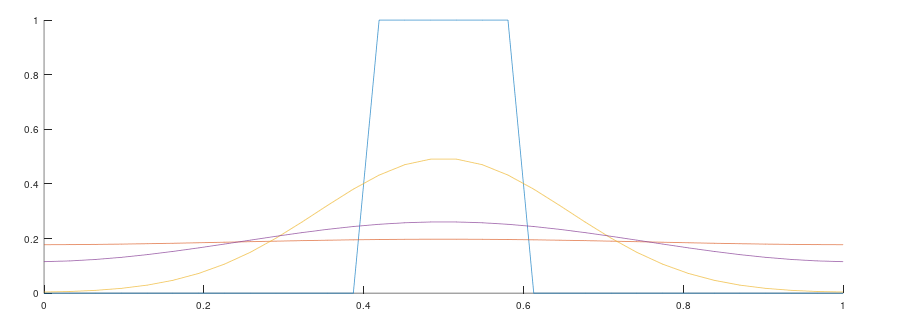
\includegraphics[width=\textwidth]{diff}
    \end{figure}
    \tiny
    A few snapshots of the diffusion. Note how because of the periodic BCs,
    all the ``particles'' is contained in the interval. A particle that goes
    out to the right, comes in from the left side, so the macroscopic distribution
    will flatten out to a certain constant level, and never reach zero as with
    the same equation solved over all of $\mathbb R$.
\end{frame}

\begin{frame}
    \begin{figure}
        \centering
        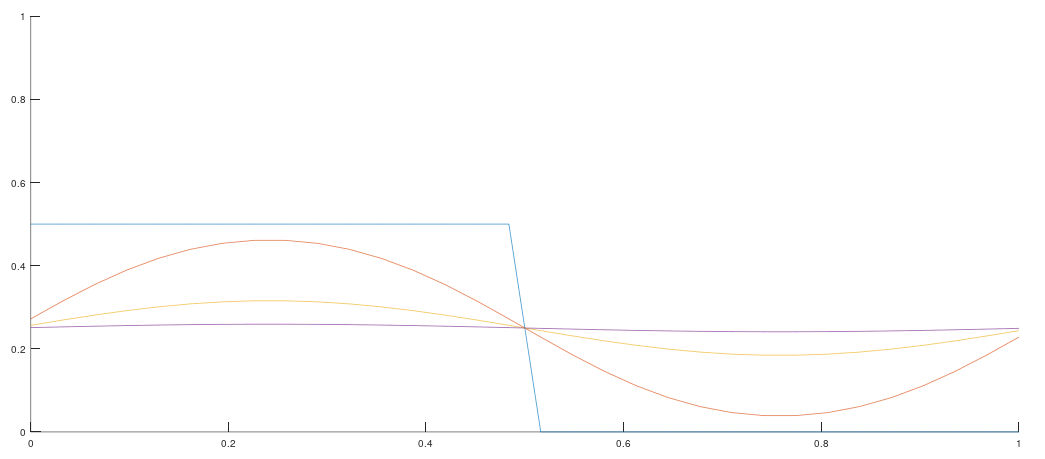
\includegraphics[width=\textwidth]{diff2}
    \end{figure}
    \tiny
    A few snapshots of the diffusion with the initial value
    \texttt{u0 = 0.5 * (x <= L/2)}. Here it is even more obvious that some
    particles are flowing out the left side and in the right side.
\end{frame}

\end{document}
